\tcbsection{Organization for Student Learning}
\subsection{A1 School Purpose Criterion}
\subsubsection{Beliefs and Philosophy}

\indicator{The written mission and vision reflects the beliefs and philosophy of the school and its constituency.}

\prompt{Evaluate the written purpose in relationship to the beliefs and philosophy of the school and its constituency served.}

\begin{findings}
CMIS has a clear Vision, Mission and Student Learner Outcomes that reflect the beliefs and philosophy of the school. These are widely published and easily visible to the community. \href{http://cmis.ac.th/about/vision}{CMIS Vision and Mission}
 
{\centering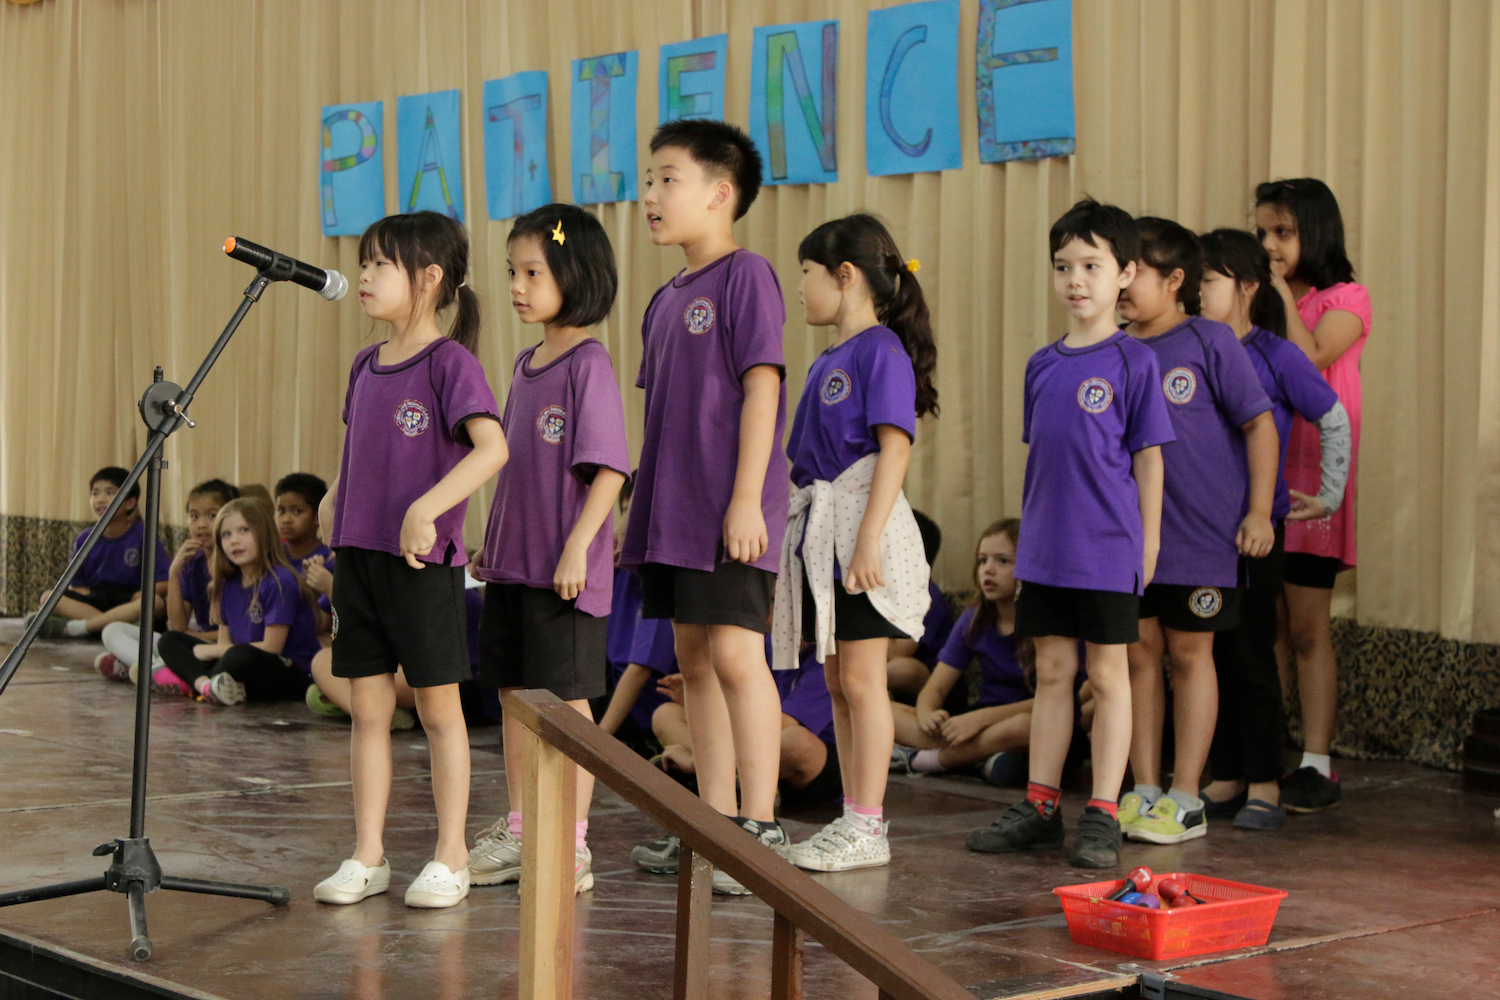
\includegraphics[width=\textwidth]{4_1_1_b.jpg}}

CMIS stakeholders strive to continuously uphold the mission of providing educational excellence, in a caring Christian community that celebrates and respects diversity. \href{https://docs.google.com/a/cmis.ac.th/presentation/d/1EJ3zT-xwUj2W--v5mTN6xWOqewtvhXrhTxXuoR1HyAg/edit?usp=sharing}{CMIS Mission Statement Project} 

The current version of our mission statement resulted from the work of a committee of board members, administrators, teachers, and parents in 2014-2015. Though recently updated, the CMIS mission is still aligned to the historical values of the school.

This year, our student learner outcomes posters displayed around campus were designed and created by our grade 6-12 students. Who We Are Student Poster Competition 

\minor{So what...}

CMIS has a clear Vision, Mission and Student Learner Outcomes that reflect the overall goal of the school community. These are continuously referred to and well known throughout the community. 

We need to find more opportunities to receive feedback from parents on the relevancy of our school “purpose” so we can remain confident that it reflects the beliefs and philosophy of the whole school and its constituency.
\end{findings}

\subsubsection{Purpose, Schoolwide Learner Outcomes, and Profile Data}

\indicator{The student/community profile data and identified global competencies have impacted the development of the school’s vision, mission, and schoolwide learner outcomes.}

\prompt{Evaluate the degree to which the development of the school’s vision, mission, and schoolwide learner outcomes have been impacted by pertinent student/community profile data and identified global competencies, and current educational research}

\begin{findings}
Our community profile data has greatly impacted the development of the\href{http://cmis.ac.th/about/vision}{ CMIS’ Mission, Vision and Student Learning Outcomes Statement}:

{\centering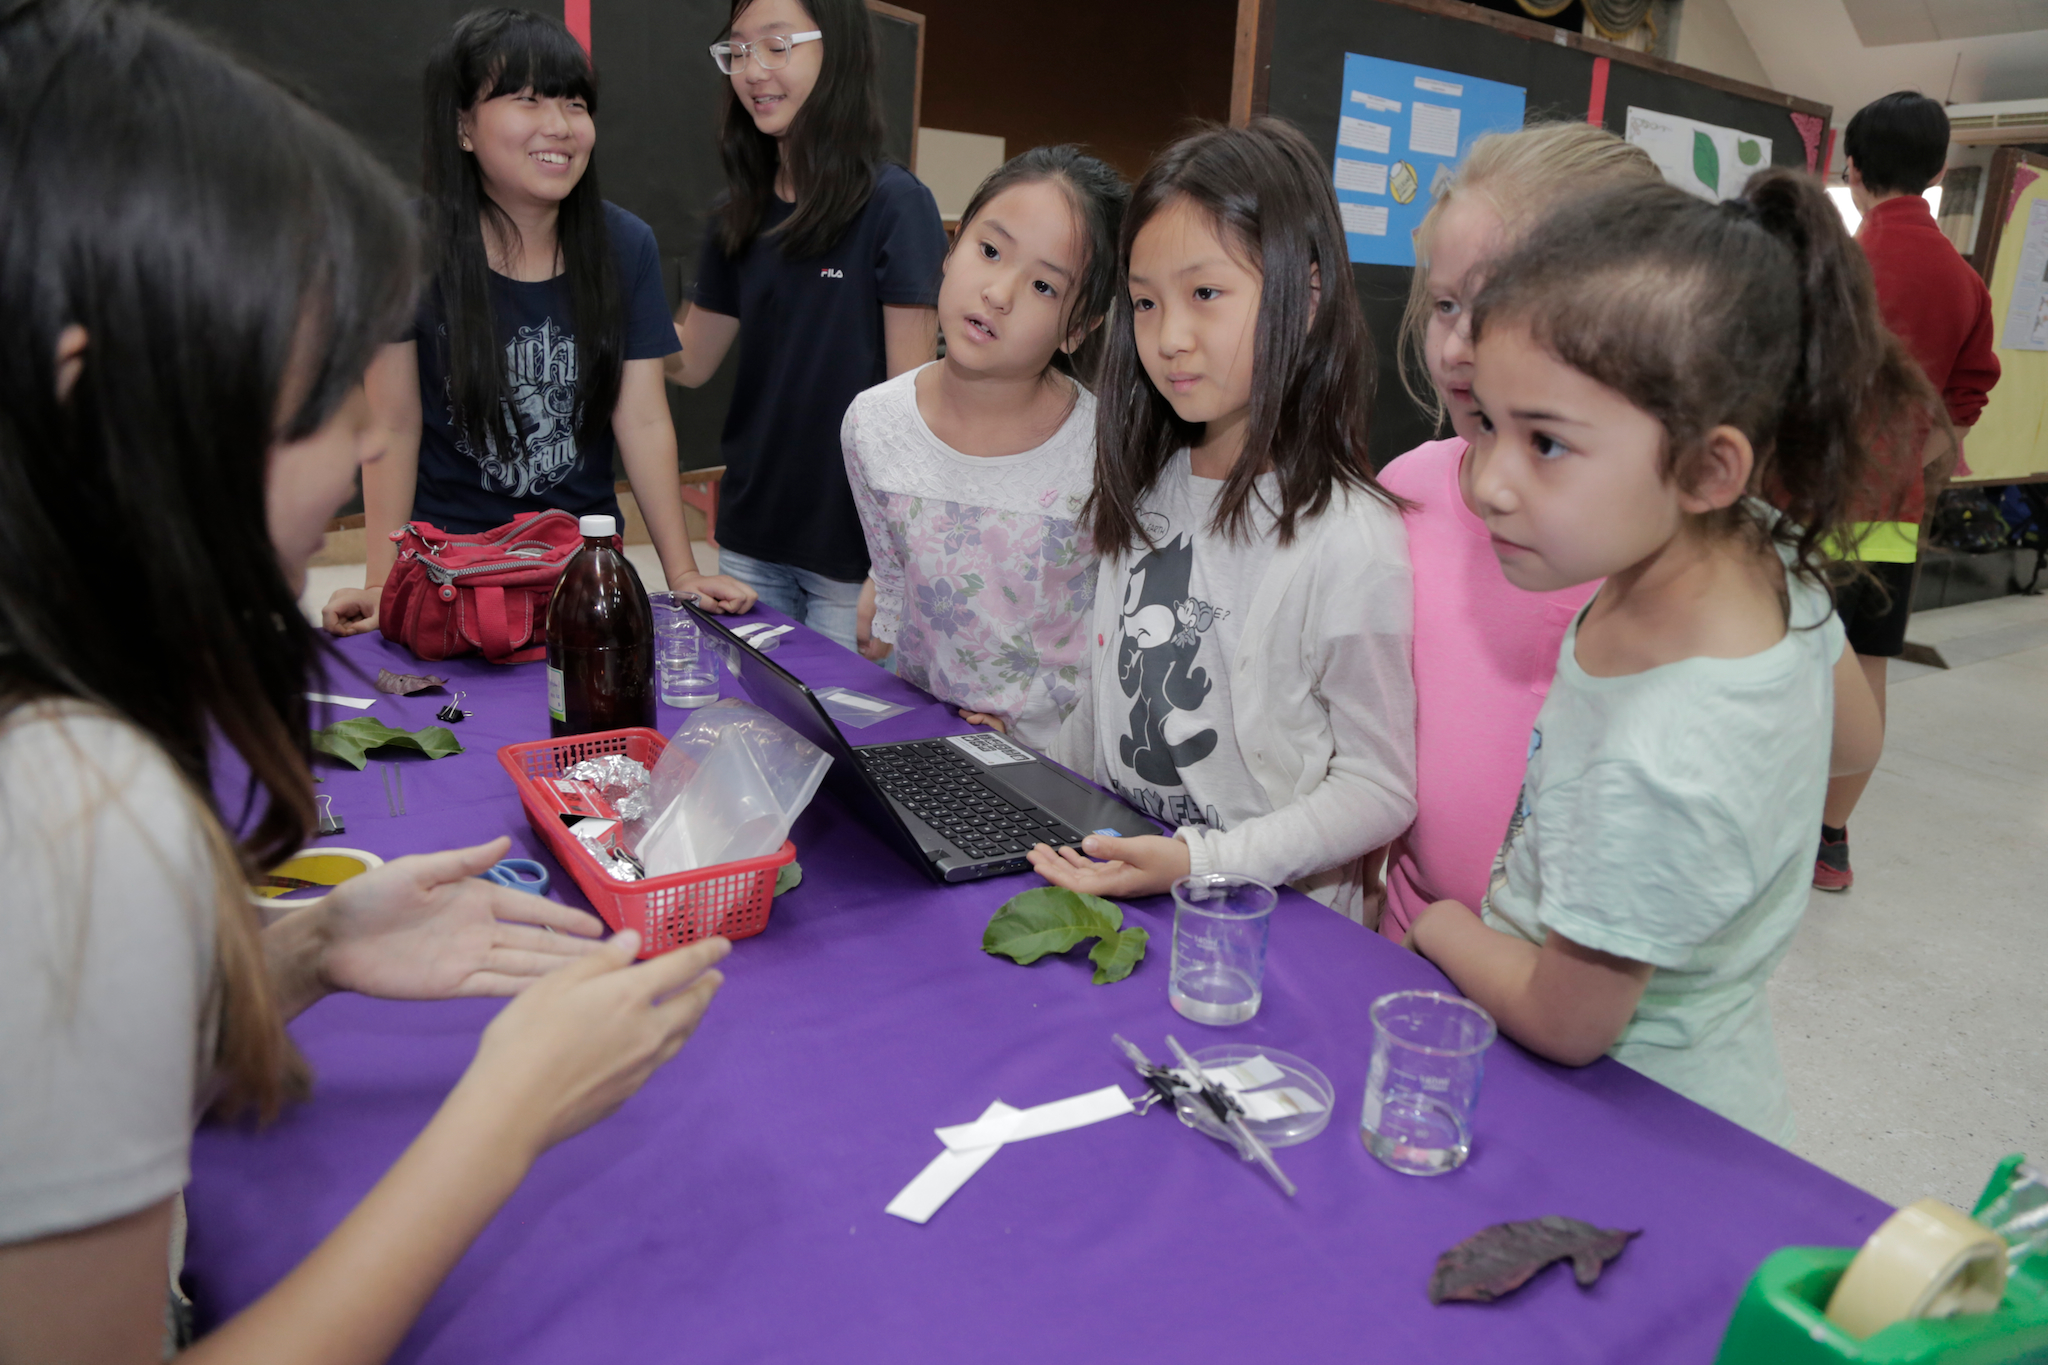
\includegraphics[width=\textwidth]{4_1_1_c.jpg}}

Our \href{https://docs.google.com/document/d/1bIbV9pgGz2vpXYJdnRzL_Od5PS35egy7lgBOBuszgD4/edit}{Student Learner Outcomes} (SLOs) were modified from their original format as Educational Objectives in 2015 to better recognize our diverse student population (32 different nationalities), embrace our global citizenship responsibilities, and include updated 21st century skills. These outcomes were reviewed with all students at the beginning of the 2016-2017 school year and their interpretations were displayed as posters across campus. \href{https://docs.google.com/a/cmis.ac.th/presentation/d/1bdi1LZUjWbGKOyB0XR9CGyoY2xLY39SZVKhiHTIJGxc/edit?usp=sharing}{Student Poster Competition}.

Our diverse group of \href{http://www.cmis.ac.th/about/faculty}{highly qualified educators} originating from over 12 different countries reflect the different cultures and nationalities of our community. Our additional support staff positions also reflect our efforts to meet our community needs (examples: Korean liaison and student spiritual advisor).

CMIS addresses global competencies in a variety of ways beyond the school mission and SLOs. Academically, CMIS students are engaged in learning standards that are internationally benchmarked and rigorous. \href{https://drive.google.com/drive/folders/0ByVFfrm0zfolMVRQYmI1aGlRNDQ}{CMIS Teaching Standards K-12}.

CMIS students have multiple opportunities to engage in school activities and events that require global understanding (e.g. \href{http://gallery.cmis.ac.th/zp-core/full-image.php?a=2010-2011/thai-day-2011/website&i=_mg_3802-version-2.jpg&q=100&wmk=\%21&dsp=Protected\%20view&check=788a1e55c231186711f8dcc0876f4efd0daa0880}{Thai Day}) celebration of diversity (\href{http://gallery.cmis.ac.th/zp-core/full-image.php?a=2013-2014/international_day&i=_MG_6129.jpg&q=100&wmk=\%21&dsp=Protected\%20view&check=788a1e55c231186711f8dcc0876f4efd0daa0880}{International Day}) sharing multiple perspectives (e.g. \href{https://www.nhd.org/}{National History Day}) and using multilingual skills (e.g. Model United Nations Club). 

{\centering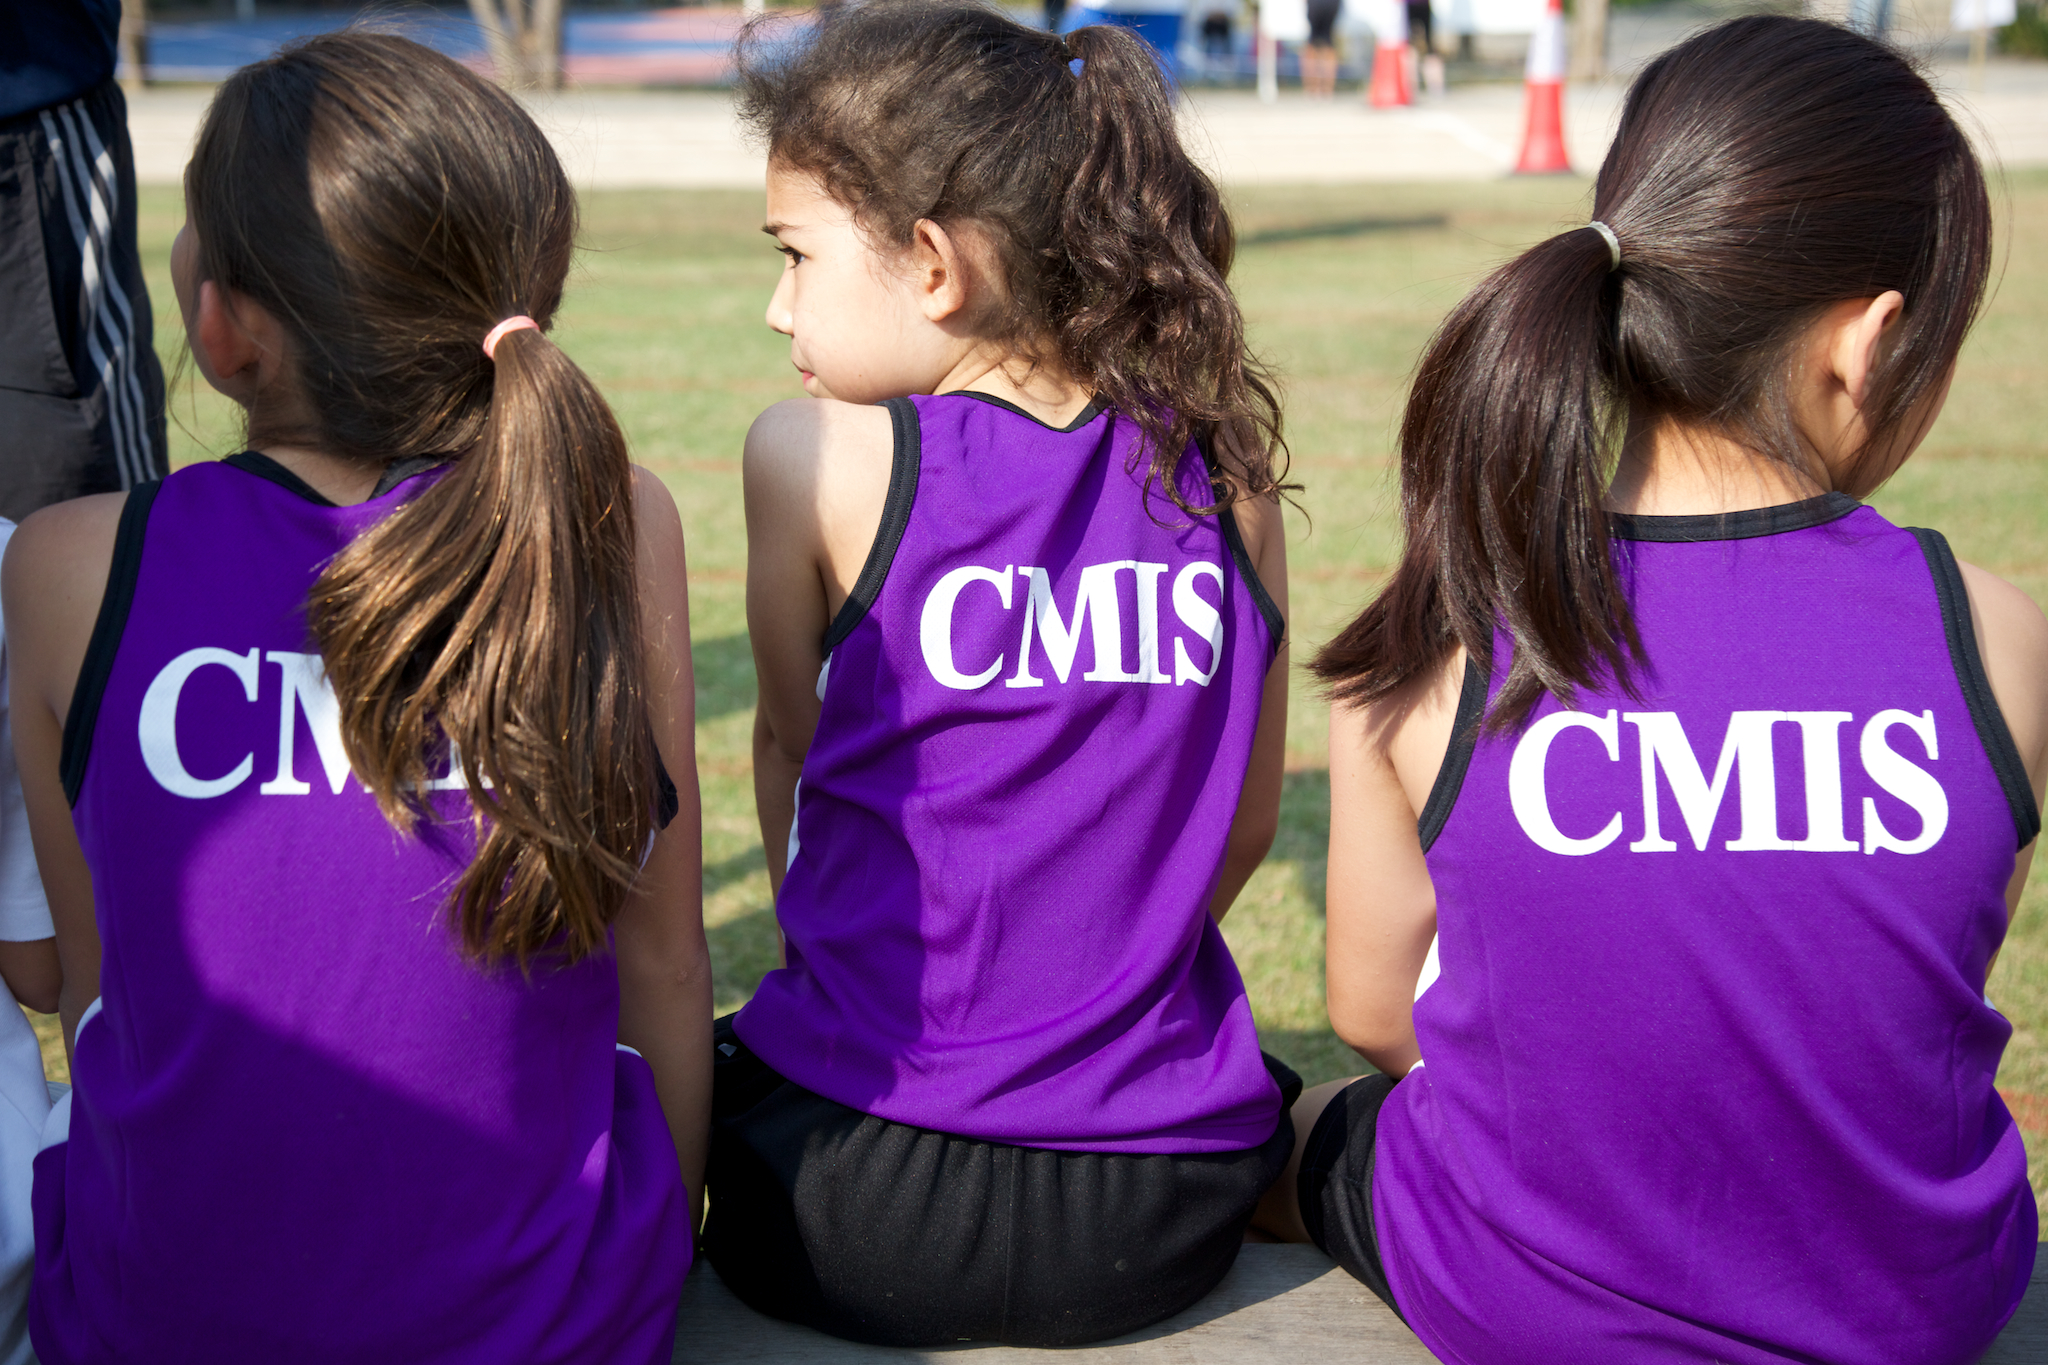
\includegraphics[width=\textwidth]{4_1_1_a.jpg}}

We use globally recognized, research-based standardized tests to identify and assess student needs (e.g, DRA, MAPS, PSAT, and SAT). 

CMIS extracurricular activities (Student Life Beyond The Classroom) emphasize the development of critical thinking skills, the ability to solve problems, and the utilization of effective communication skills. \href{http://blogs.cmis.ac.th/eagles/}{Student Life Beyond the Classroom}

CMIS students participate in community service projects at all three divisions (ES, MS and HS) to promote responsibly in action and service to improve conditions both locally and globally. Examples include Elementary School Thanksgiving Drive for Hope House (local orphanage), \href{https://drive.google.com/a/cmis.ac.th/file/d/0B7jcj1TRcFEGNEtqR3hUSW5QVHM/view?usp=sharing}{Middle School Activity Day} at Hope House and High School \href{http://blogs.cmis.ac.th/community-service/}{community service projects}.

\minor{So what...}

There are many ways in which our school can demonstrate how our vision, mission, and schoolwide learner outcomes have been impacted by pertinent student and community profile data, identified global competencies, and current educational research. 
As our student and community profile is constantly changing, we need to always ensure that we keep abreast of these changes and modify our goals accordingly.
\end{findings}

{\centering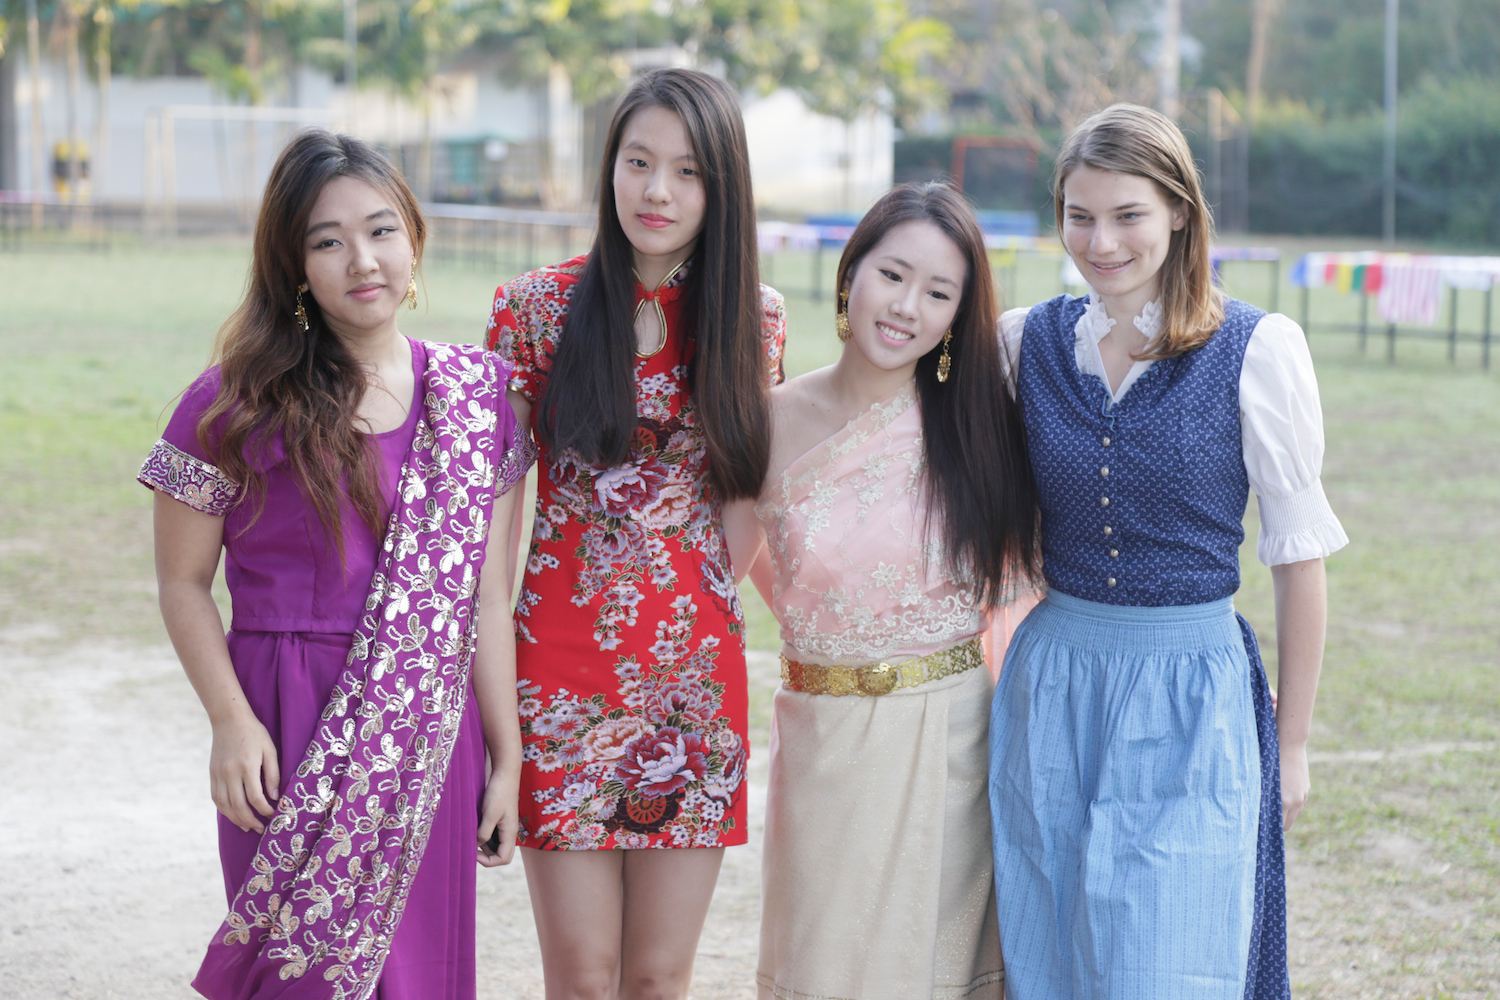
\includegraphics[width=\textwidth]{chapter4_A1.jpg}}

\subsubsection{Involvement of All}

\indicator{The school has a process for involving representatives of the entire school community in the defining of global competencies and in the development/refinement of the core values, mission, vision, and schoolwide learner outcomes.  }

\prompt{Evaluate the processes 1) to ensure the involvement of representatives from the entire school community in the defining of global competencies and the development/refinement of the core values vision, mission, and schoolwide learner outcomes and 2) to determine their effectiveness.}

\begin{findings}
CMIS has several processes for involving representatives of the entire school community in the development/refinement of the core values and schoolwide learner outcomes:

“Teacher Table Talk” sessions are often held during staff development, early release days to capture insights and suggestions about the effectiveness of the CMIS Mission and Student Learner Outcomes.  Example: \href{https://drive.google.com/a/cmis.ac.th/file/d/0ByVFfrm0zfolbHNvSWhVWmJYU3M/view?usp=sharing}{Teacher Table Talk Activity} 

ES students and staff create and participate in monthly \href{https://docs.google.com/a/cmis.ac.th/document/d/1Mv1xjTpbY36naur8SDt9GanKNfR7YtYVL-bWwGLPSHo/edit?usp=sharing}{virtue assemblies} that review and reinforce our school mission, vision and SLO’s. Parents are also invited to attend these events.

{\centering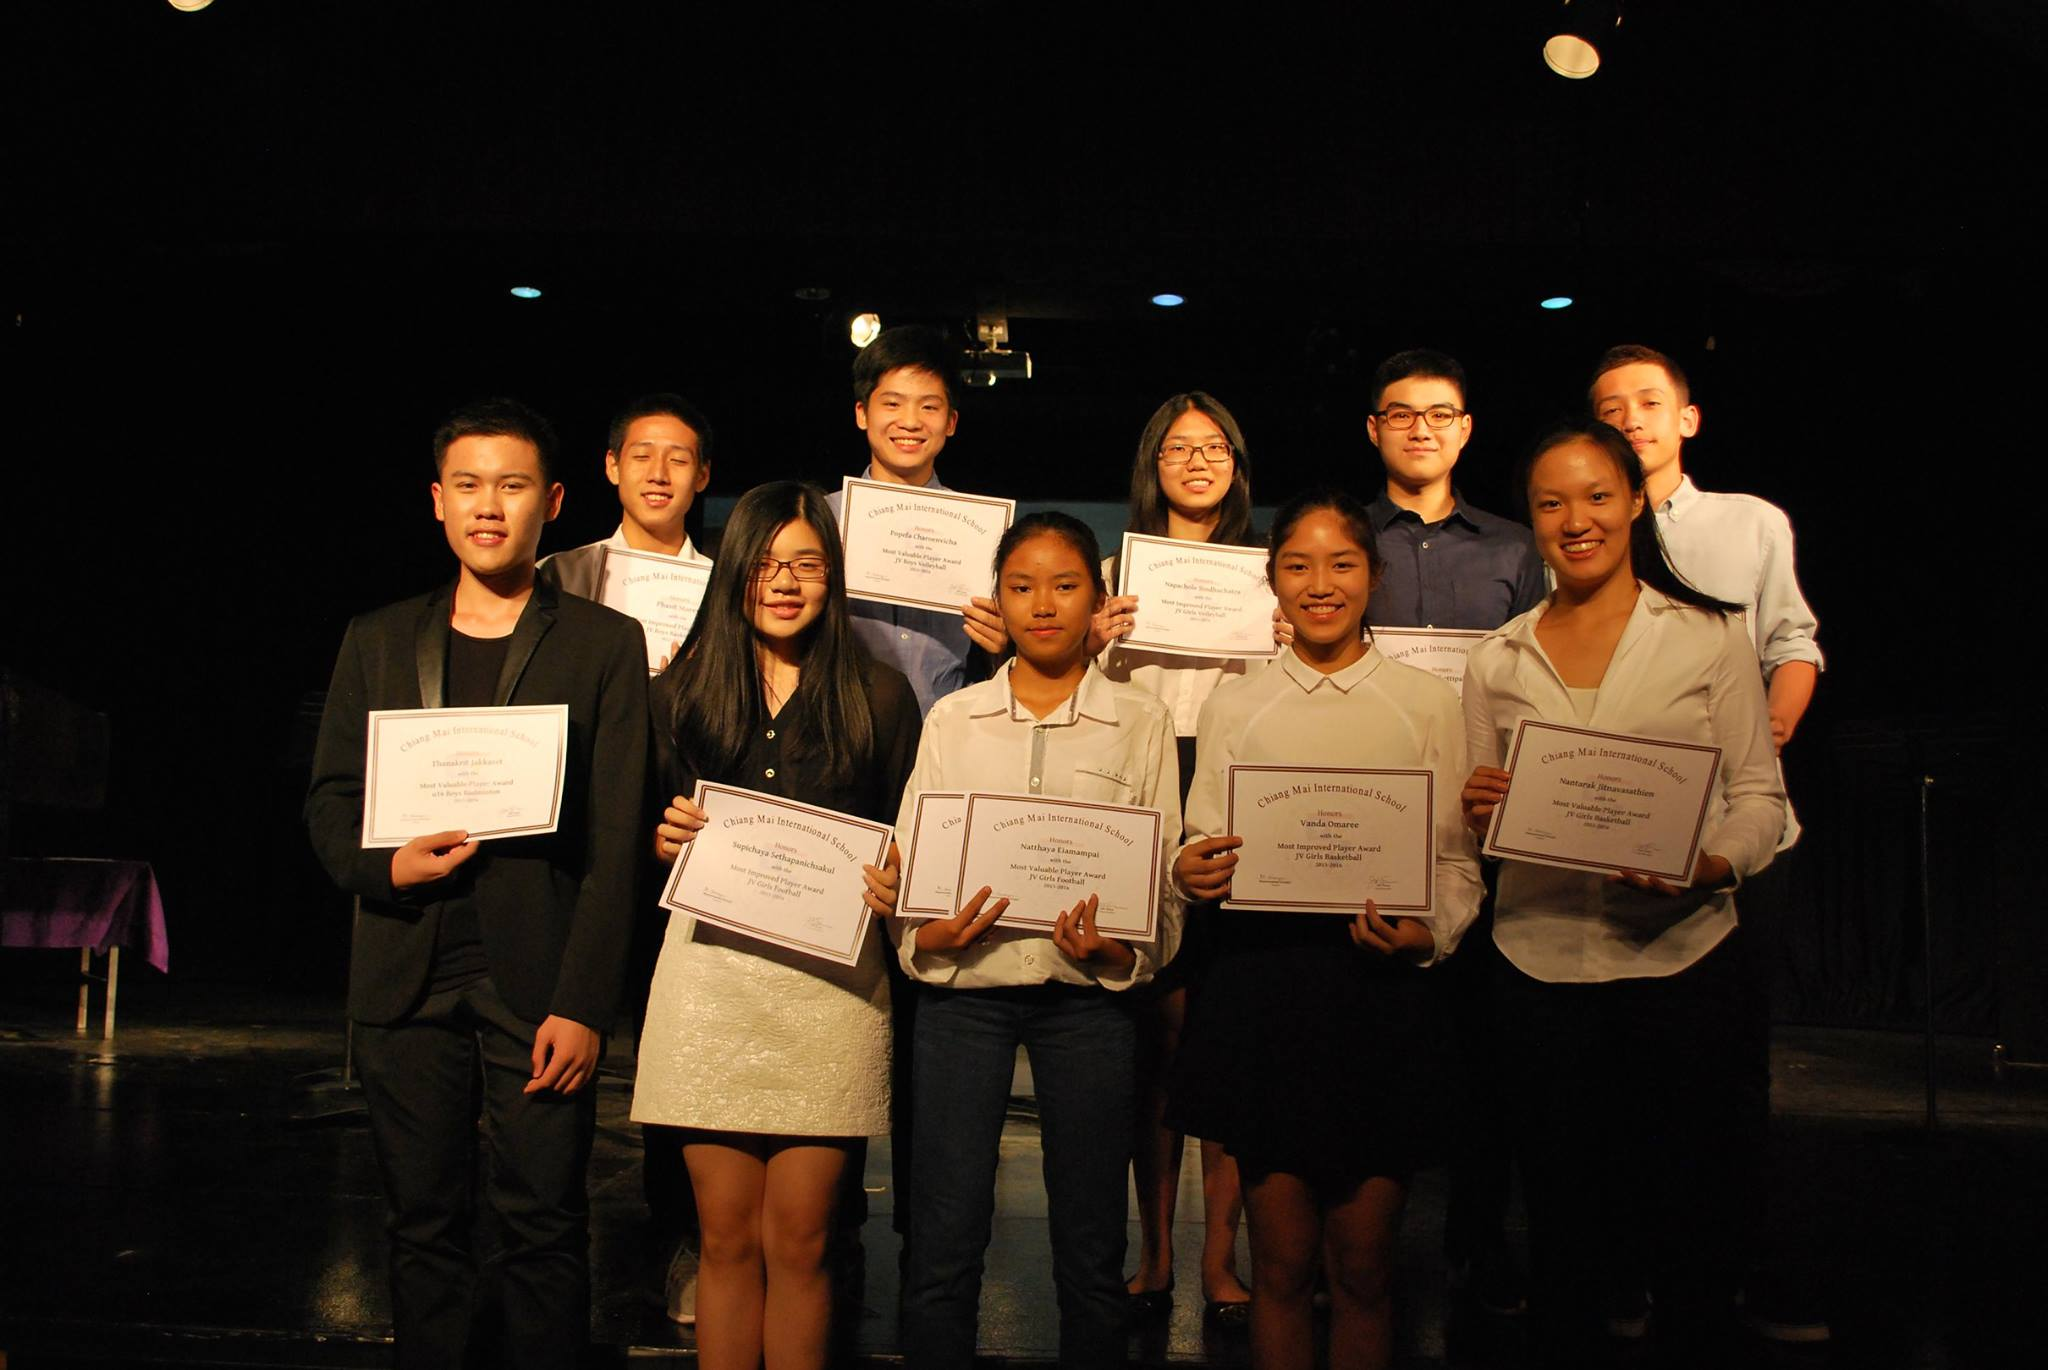
\includegraphics[width=\textwidth]{4_1_1_d.jpg}}

MS and HS Students are encouraged to review our vision, mission, and schoolwide learner outcomes during bi-weekly communication group activities. Communication group have approximately 5-7 students and a teacher leader. This group remains together as a team every year throughout MS and HS.
 
This year, our student learner outcomes posters displayed around campus were designed and created by our grade 6-12 students. \href{https://docs.google.com/a/cmis.ac.th/document/d/1x29XpA7Ro2Xav3JFY0k9F2O22qZi4Yo48hVTYkvhoGM/edit?usp=sharing}{Who We Are Student Poster Competition}.

Several of our student-led clubs involve the defining of global competencies, development/refinement of CMIS core values vision, mission, and schoolwide learner outcomes  (example: CMIS Environmental Club and National Honors Society).

CMIS \href{https://docs.google.com/a/cmis.ac.th/forms/d/16Gbd3MzQOXtjjZ2dG460xw5SHG_eohMIKet3lxYUdAY/prefill}{family surveys} are conducted once a year to solicit feedback from staff, students and parents. The survey gathers data to monitor the effectiveness of CMIS in relation to its mission, vision, and SLO’s. The survey data is analyzed, summarized and used to create goals for improvement. These goals are then shared with each constituency group at the beginning of the year and monitored for progress throughout the year. Example: \href{https://docs.google.com/a/cmis.ac.th/document/d/10w_OSr00xntX42ShaPk4PiNu9FjKP2OgA3g6CKjmEFc/edit?usp=sharing}{Student feedback about cafeteria}.

Our \href{http://blogs.cmis.ac.th/ptg/about/}{CMIS Parent Teacher Leadership Team}- assists and supports the school in the development/refinement of the core values, mission, vision, and schoolwide learner outcomes. This team focuses on this role during monthly meetings with the superintendent, as a leadership team, and during monthly parent meetings that the school management team always attends.

\minor{So what...}

CMIS strives to involve representatives of the entire school community in the development/refinement of the core values and schoolwide learner outcomes.

We believe that we can seek further involvement, and we are trying to reach out and include more involvement with our community-outside of our immediate parent group (examples of progress: reaching out to rotary club and US Consulate).
\end{findings}

\subsubsection{Consistency of Purpose, Schoolwide Learner Outcomes, and Program}

\indicator{There is a strong degree of consistency between the school core values, vision, mission, the schoolwide learner outcomes, and the school program that reflects the school’s explanation of global competencies.}

\prompt{Provide a range of examples that the school vision, mission, schoolwide learner outcomes, and program are consistent. with the school’s explanation of global competencies.}

\begin{findings}
CMIS believes that a global competency doesn't always have to be about world events or other countries, but rather about how to live in the world. Learning how to listen, how to disagree respectfully, how to encourage, and how to collaborate are several elements of a global education that all students need.

The CMIS \href{http://cmis.ac.th/about/vision}{Mission Statement}, \href{http://cmis.ac.th/about/vision}{Student Learner Outcomes}, and school programs are closely related to our goal to equip international students for lives of learning and positive contributions both locally and globally (See \href{http://cmis.ac.th/about/vision}{Who We Are} on website).

CMIS adopted K-12 standards in 2013 that are closely aligned with the school’s mission of academic excellence through rigor, coherence and focus. Our instruction is inquiry-based, which also supports the CMIS key learner outcomes for our students. 

Our grade 6-12 initiative of the 1:1 chromebook reflects our mission to enhance student global proficiency through hands-on, student-centered, and meaningful technology integration. 

Our 2016 \href{https://docs.google.com/a/cmis.ac.th/presentation/d/1xmLAJD96klLrjiBPwCoOMoKmbclYqpIMWaifytzFMgk/edit?usp=sharing}{chromebook survey} results indicated that 73\% of our students felt that the chromebooks increased their ability to demonstrate their learning and 77\% felt that the chromebooks helped them to be more productive. The survey also confirmed how the chromebooks were being used to support essential global competency skills (e,g, presenting, communicating, organizing, researching, and collaborating)

The results of our \href{https://drive.google.com/a/cmis.ac.th/file/d/0B71_pYxcTLo-RlZxQzQyc0NqUFU/view?usp=sharing}{community surveys} confirm that 95\% of our parents parents believe that CMIS provides a high quality education: educational excellence in a caring Christian community that respects and celebrates diversity.

CMIS believes that a global education is not a separate subject or a single lesson; it is a necessary part of all education, for all people. Global education allows a shift in perspective, which provides opportunities for both students and teachers to grow and develop as humans equipped with an understanding of their roles in a complex world.

Some specific teams and staff positions in place to help ensure the promotion of global competency:

\begin{itemize}
\item \href{http://blogs.cmis.ac.th/eagles/}{Student Life Beyond the Classroom} Team
\item Spiritual and Community Service Advisor
\item Spiritual Life Committee
\item \href{http://blogs.cmis.ac.th/ptg/about/}{Parent Teacher Group} Leadership Team
\item Middle School and High School Communication Groups
\item Elementary, Middle, and High School Counselors
\item ES, MS, and HS Student Success Team
\end{itemize}

\minor{So what...}

We have a strong degree of consistency between the school core values, vision, mission, the schoolwide learner outcomes, and the school programs that reflects the school’s explanation of global competencies.

We are trying to move away from the commercial definition of global competency and move towards a more student-centered definition that focuses on authentic opportunities for our community to grow together in a caring community as proactive human beings (i.e. \href{https://drive.google.com/a/cmis.ac.th/file/d/0B0TYmzaZNi3fOF9RQkRqLV9saUE/view?usp=sharing}{Great Kindness Challenge Week}).
\end{findings}

\subsubsection{Communication about Vision, Mission, and Schoolwide Learner Outcomes}

\indicator{The school has means to publicize the \href{http://cmis.ac.th/about/vision}{vision, mission, and schoolwide learner outcomes} to the students, parents, and other members of the school community.}

\prompt{Examine the effectiveness of the means to publicize the purpose and the schoolwide learner outcomes to the students, parents, and other members of the school community.}

\begin{findings}
CMIS has various means to communicate its Vision, Mission Statement and the Student Learner Outcomes to the entire school community:

The CMIS Student Handbook, part of the annual Student Planner, contains information that focuses on our school mission to develop learners who can pursue personal and academic goals, based on academic excellence and strong moral foundations. Link to \href{https://docs.google.com/document/d/1bIbV9pgGz2vpXYJdnRzL_Od5PS35egy7lgBOBuszgD4/edit}{Student Handbook}

Our Vision, Mission and Student Learner Outcomes are displayed prominently throughout campus (examples: student posters and Bible verse banners). 

CMIS publicizes the school vision, mission and student learner outcomes through the CMIS website, accessible to the public and a portal accessible to all parents, students and faculty. It is also included as a footer on all administrative e-mails.  Link to \href{http://cmis.ac.th/about/vision}{Who We Are} on website

School administration always reiterates the school philosophy at all school wide events (e.g. new family orientation, back-to-school night, assemblies). 

As a Christian school, we provide a variety of schoolwide and volunteer opportunities for our community to interact with the Christian ethos, while also respecting the religious diversity of our community (e.g. school-wide Christmas and Easter assemblies, lunchtime bible study groups, and Christian Club Picnic).

Our PTG team reinforces the school vision, mission and student learner outcomes throughout their coffee morning meetings for new families at the beginning of each school year. 

Our board of directors uses the vision and mission in their agenda planning template and uses it as a point of reference throughout their monthly meetings. These meetings are then \href{http://blogs.cmis.ac.th/ptg/public-board-minutes/}{summarized} and shared with our CMIS community on our website.

Our school management team regularly asks for feedback on the effectiveness of our school goals with parents at our PTG meetings, with our staff during our monthly professional development and divisional meetings.

We reflect upon our school goals with our grade 6-12 students during their bi-weekly communications groups and with our elementary students during their and monthly virtue assemblies.

Our teacher leadership team utilize the \href{https://drive.google.com/a/cmis.ac.th/file/d/0ByVFfrm0zfolT25VTjZZRzlXQjA/view?usp=sharing}{meeting wise agenda format} that requires participants to reflect on the objectives of the department meeting in relation to our school goals.

In September a \href{https://docs.google.com/a/cmis.ac.th/presentation/d/1bdi1LZUjWbGKOyB0XR9CGyoY2xLY39SZVKhiHTIJGxc/edit?usp=sharing}{student art competition} was initiated and the student illustration entries were used to better communicate the CMIS vision, mission and student learner outcomes.

Our CMIS weekly newsletter, blogs and \href{https://www.facebook.com/cmis.th/}{Facebook updates} are other effective ways we communicate our Vision, Mission, and Student Learner Outcomes to our community. 

\minor{So what...}

We work hard to publicize the vision, mission, and schoolwide learner outcomes to the students, parents, and other members of our school community.

We are trying to think of more ways of communicating our message in an easier to understand format. Having our students illustrate our philosophy has been very useful, especially with our community members whose english is not their first language.
\end{findings}

\subsubsection{Regular Review/Revision}

\indicator{The school has a process for regular review/revision of the school’s vision, mission, and  schoolwide learner outcomes based on current and future learner needs and other local and global trends and conditions.}

\prompt{Evaluate the effectiveness of the regular process for review/revision of the core beliefs, school vision, mission, and the schoolwide learner outcomes. Include the degree to which the review/revision process addresses current and future learner needs and other local and global trends and conditions.}

\begin{findings}
CMIS has a process for regular review of the CMIS core beliefs based on student needs, global, local needs, and other trends and community conditions.

Our school mission was updated in 2014 and the modified version was formulated by our staff based on current students needs, global and local needs, and other trends and community condition. 

Our Student Learner Outcomes were modified from their original format as Educational Objectives in 2015 to better recognize our diverse community, further embrace students future needs, and include updated global skills. These outcomes were reviewed with the whole community at the beginning of the 2016-2017 school year and student interpretations were displayed as posters across campus. \href{https://docs.google.com/a/cmis.ac.th/presentation/d/1bdi1LZUjWbGKOyB0XR9CGyoY2xLY39SZVKhiHTIJGxc/edit?usp=sharing}{Student Poster Competition}

Each year, CMIS sends an annual community survey (parents, teachers, and students grades 4-12) to solicit perception data related to our effectiveness of implementing our school mission and student learner outcome goals.

\minor{So what...}

As the school’s mission statement and SLOs were recently updated, there has not yet been any rigorous effort to revise them.  However, as CMIS continues to grow and identify innovative ways to enhance teaching and learning, the statement and the SLO’s will be re-evaluated and revised to mirror the diverse needs of our CMIS community.

The CMIS Board has been developing an evaluation instrument for administrators and board members to ensure fidelity to mission, vision, and schoolwide learner outcomes.  Concurrently, the CMIS Board is currently identifying indicators to determine the academic quality and fiscal health of the school. 
\end{findings}

\subsubsection{Conclusions}

\prompt{Comment on the degree to which this criterion is being addressed.}

\begin{findings}

The findings suggest that CMIS addresses this criterion to a high degree. In an effort to increase student achievement further in this area CMIS plans to:

\minor{Maintain and Monitor}

\begin{itemize}
\item Processes and policies that have a strong degree of consistency between the school core values, vision, mission, and the schoolwide learner outcomes.
\item Regular opportunities to continuously communicate school goals with the community
\end{itemize}

\minor{Investigate Better Practice}

\begin{itemize}
\item Ways to communicate CMIS goals in easy to comprehend formats
\item Keeping current with community profile and modifying CMIS goals accordingly.
\end{itemize}

\end{findings}
